\documentclass[xcolor=pdftex,dvipsnames,table,aspectratio=169]{beamer}
%\documentclass[xcolor=pdftex,dvipsnames,table,handout,aspectratio=169]{beamer}

%\setbeameroption{show notes}

\usepackage{bm,graphicx,multirow,amsmath,tikz} %fancybox,
\usepackage{color}%,textpos}
\usepackage[round]{natbib}
\usepackage[normalem]{ulem}
\usepackage{hyperref}
\usepackage{lastpage}
\usepackage{array}
\usepackage{color}
\usepackage{framed}
\usepackage{hyperref}

% Define Western colours
\definecolor{western}{rgb}{.306,.152,.524}
\definecolor{westerngray}{rgb}{.512,.508,.524}

%% Define BEAMER colours
\setbeamercolor{frametitle}{bg=western,fg=white}
\setbeamercolor{framesubtitle}{bg=western,fg=black}
\setbeamercolor{title}{fg=white,bg=western}
\setbeamercolor{author}{fg=white,bg=western}
\setbeamercolor{institute}{fg=white,bg=western}
\setbeamercolor{date}{fg=white,bg=western}

%% Set BEAMER fonts
\setbeamerfont{title}{shape=\bf}
\setbeamerfont{frametitle}{shape=\sc,size=\Large}
\setbeamerfont{framesubtitle}{shape=\sc,size=\Large}
\setbeamerfont{footline}{shape=\sc}

%% Define BEAMER toc
\setbeamercolor{section in toc}{fg=western}
\setbeamercolor{subsection in toc}{fg=westerngray}
\setbeamertemplate{sections/subsections in toc}[ball]

%% Define BEAMER background
\setbeamercolor{background canvas}{bg=white}

%% Define BEAMER footer
\setbeamertemplate{navigation symbols}{}
\setbeamercolor{footline}{fg=white,bg=western}
\setbeamertemplate{footline}{%
  \begin{beamercolorbox}[wd=\paperwidth]{footline}
    \vskip5pt

    \raisebox{.05in}{
      \scriptsize{\bf \insertshorttitle}
    }
    \hfill
    \raisebox{.05in}{
      \scriptsize{\bf \insertframenumber/\inserttotalframenumber} 
    }
    \hspace{5pt}

    \vskip5pt
  \end{beamercolorbox}
}

%% Define BLOCK environment
\setbeamercolor{block title}{fg=western}
\setbeamerfont{block title}{series=\bfseries}

%% Define ENUMERATE and ITEMIZE environements
\setbeamertemplate{itemize item}[ball]
\setbeamertemplate{enumerate item}[ball]
\setbeamercolor{item projected}{bg=western}

%% Define BEAMER toc
\setbeamercolor{sections/subsections in toc}{fg=blue!75}
\setbeamertemplate{sections/subsections in toc}[ball]

% %% Define SECTION openings
% \AtBeginSection[]{
%   \begin{frame}{\insertshorttitle}
%     \tableofcontents[currentsection,subsectionstyle=hide/hide/hide]
    
%   \end{frame}
% }

%% Define BEAMER frametitle
\addtobeamertemplate{frametitle}{
   \let\insertframetitle\insertsectionhead}{}
\addtobeamertemplate{frametitle}{
   \let\insertframesubtitle\insertsubsectionhead}{}


\makeatletter
  \CheckCommand*\beamer@checkframetitle{\@ifnextchar\bgroup\beamer@inlineframetitle{}}
  \renewcommand*\beamer@checkframetitle{\global\let\beamer@frametitle\relax\@ifnextchar\bgroup\beamer@inlineframetitle{}}
\makeatother

% Define counters for example and exercise
\newcounter{example}
\newcounter{exercise}

% Define example and exercise commands
\renewcommand{\example}
{\stepcounter{example}Example \lecturenum.\arabic{example}}
\newcommand{\examplectd}
{Example \lecturenum.\arabic{example}\ ctd}
\newcommand{\exercise}
{\stepcounter{exercise}Exercise \lecturenum.\arabic{exercise}}
\newcommand{\exercisectd}
{Exercise \lecturenum.\arabic{exercise}\ ctd}

\newcommand{\lecturenum}{13}

\title[SS2857]{Probability and Statistics I}
\subtitle{\lecturenum. Discrete Distributions: Summary Exercise}

\date{}

%% Add logo
% \titlegraphic{\includegraphics[height=2cm]{../uwo_logo_reversed}}

%% Initialize R


\begin{document}

{
\setbeamertemplate{footline}{}
\setbeamercolor{background canvas}{bg=western}

\begin{frame}
  \addtocounter{framenumber}{-1}

  \maketitle
\end{frame}
}



\begin{frame}

\begin{center}
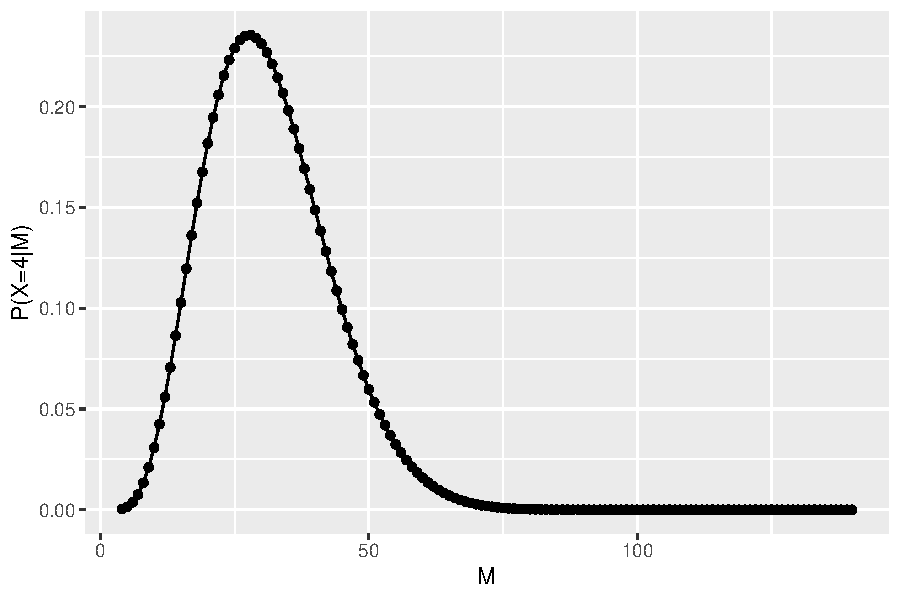
\includegraphics[height = .8\textheight]{figure/plot1-1}
\end{center}

\end{frame}

\begin{frame}

\begin{center}
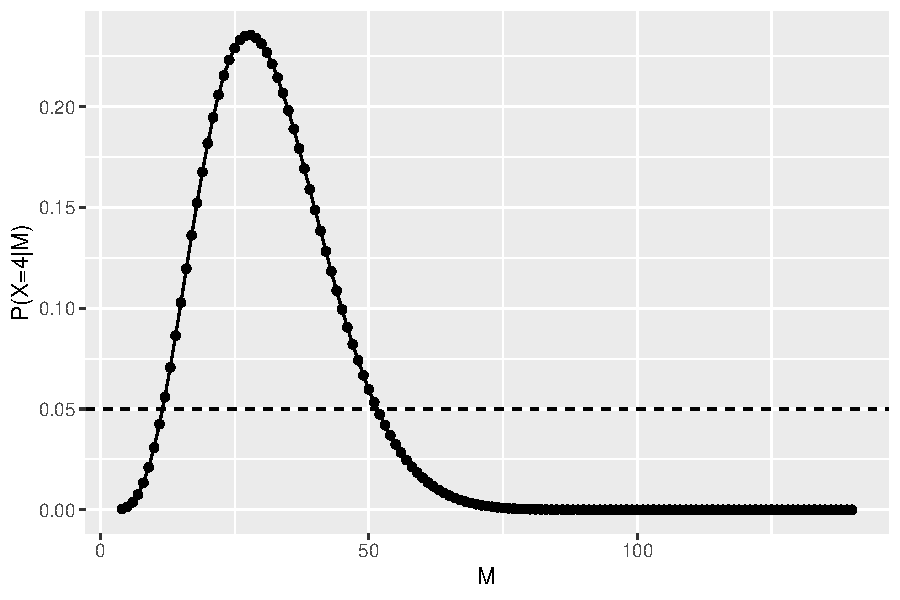
\includegraphics[height = .8\textheight]{figure/plot1-2}
\end{center}

\end{frame}

\begin{frame}

\begin{center}
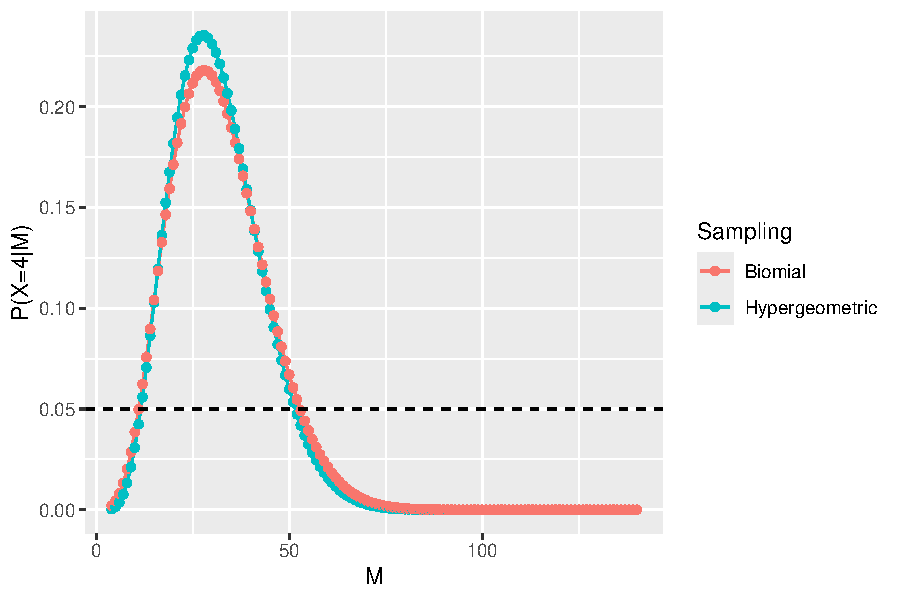
\includegraphics[height = .8\textheight]{figure/plot1-3}
\end{center}

\end{frame}

\begin{frame}

Suppose that there are 40 mint chocolate candies in the population of 140 candies and we sample candies with replacement until we select 5 mint chocolate candies.

\begin{itemize}
\item Let $X$ be the total number of candies you draw. What is the distribution of $X$?
\item What are the mean and variance of $X$?
\item Let $Z$ be the number of non-mint chocolate candies you draw. What is the distribution of $Z$?
\item What are the mean and variance of $Z$?
\item What is the relationship between $X$ and $Z$?
\end{itemize}
\end{frame}

\end{document}

